\documentclass[t]{beamer}

% set fonts
\usefonttheme{professionalfonts} % using non standard fonts for beamer
\usepackage{txfonts,mathptmx}

% set indend spacing for first and second level indentation
\setlength{\leftmargini}{0.5cm}
\setlength{\leftmarginii}{0.5cm}

% Set circles for bullets 

\setbeamertemplate{itemize items}[circle]

% increase space between text and frame name
\addtobeamertemplate{frametitle}{}{\vspace{1em}}

%Information to be included in the title page:
\title{Design Specification and RTL Coding}
\author{Nikola Petrovic}
\institute{University of Belgrade, School of Electrical Engineering}
\date{2022}



\begin{document}

\frame{\titlepage}

%%%%%%%%%%%%%%%%%%%%%%%%%%%%%%%%%%%%%%%%%%%%%%%%%%%%%%%%%%%%
\begin{frame}
\frametitle{Module Objectives}

In this module
\begin{itemize}
\item Recognize the meaning of a Design Specification using an example of a simple counter design spec
\item Implement the specified design through the RTL coding process:
\begin{itemize}
	\item Identify what Hardware Definition Languages, or HDLs, are
	\item Implement a design spec for a given design criteria
	\item Code a simple counter design given a design spec
\end{itemize}
\end{itemize}
\end{frame}

%%%%%%%%%%%%%%%%%%%%%%%%%%%%%%%%%%%%%%%%%%%%%%%%%%%%%%%%%%%%
\begin{frame}
\frametitle{Design Specification Flowchart}

\begin{figure}
\centering
    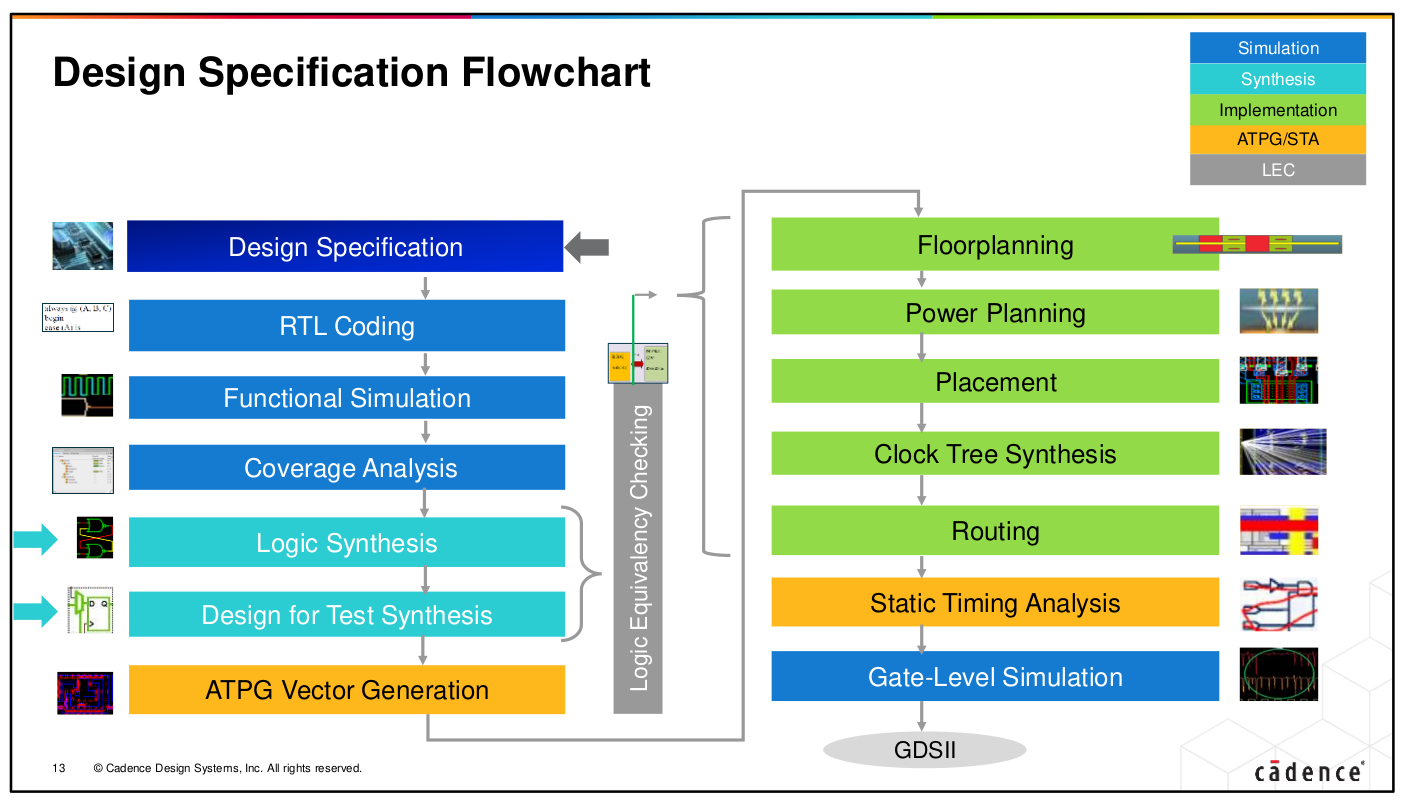
\includegraphics[width=0.95\textwidth]{map.png}
    %\caption{Overview of the Cadence RTL2GDSII flow.}
    \label{fig:map}
\end{figure}
\end{frame}

%%%%%%%%%%%%%%%%%%%%%%%%%%%%%%%%%%%%%%%%%%%%%%%%%%%%%%%%%%%%
\begin{frame}
\frametitle{What Is a Design Specification?}
A Design Specification is an explicit
set of requirements to be satisfied by
a material, product or service.

\begin{itemize}
\item An idea begins with a specification, which can be textual, graphical or sometimes a software representation.

\item It is a detailed document providing information about the characteristics of a project to set the criteria that design
engineers will need to meet to code their designs.
\end{itemize}

OVDE UBACI PRIMER NEKE SPECIFIKACIJE
OVDE UBACI PRIMER NEKE SPECIFIKACIJE

\end{frame}



%%%%%%%%%%%%%%%%%%%%%%%%%%%%%%%%%%%%%%%%%%%%%%%%%%%%%%%%%%%%
\begin{frame}
\frametitle{Example Design Spec of a Two-Bit Synchronous Binary Counter}

\begin{itemize}
\item The binary counter is an example of a simple
synchronous digital circuit. It has no data
inputs and no combinational output logic
circuit.
\item At each clock pulse, the counter takes up a
new state and thus goes through a specific
count sequence.

\item We shall now write a design spec for a binary
up-counter with two outputs which go through
the following sequence: $00 \rightarrow 01 \rightarrow 10 \rightarrow 11 \rightarrow 00 \rightarrow $ etc.

\item The counter should have the following inputs:

rst (active low),
clk

\item The counter should have the following output: count (1:0)

\item The block diagram, structure and state transition
diagram of a two-bit binary counter (built with two
D-type flip-flops) is of the following form:

\item The truth table for the circuit is as follows:

PROMENITI PRIMER
\end{itemize}


\end{frame}

%%%%%%%%%%%%%%%%%%%%%%%%%%%%%%%%%%%%%%%%%%%%%%%%%%%%%%%%%%%%
\begin{frame}
\frametitle{What Is a Hardware Description Language (HDL)?}

An HDL is a programming language with special constructs for modeling hardware concurrency and timing.

An HDL supports a design at multiple levels of abstraction:


\end{frame}


%%%%%%%%%%%%%%%%%%%%%%%%%%%%%%%%%%%%%%%%%%%%%%%%%%%%%%%%%%%%
\begin{frame}
\frametitle{Nadalje je verilog}

VERILOG DETALJNO


\end{frame}

\end{document}
